\documentclass{SKP-beamer}

% --------------------------------------------------- %
\title[Cloud File Security]{Cloud Based File Security System with Hybrid Encryption}
\subtitle{PPD-II Third Review \hspace{0.3cm} | \hspace{0.3cm} PID: 23CSEP03}
\author[23CSEP03]{PID: 23CSEP03 \\[0.3cm] \small{Ashish Kumar (2301341013)} \\[0.1cm] \small{Ashish Singh (2301341014)} \\[0.1cm] \small{Avee Ranjan (2301341016)} \\[0.1cm] \small{Ayshi Shannidhya Panda (2301341017)} \\[0.3cm] \small{Under the guidance of} \\ \textbf{Mrs. Snehanjali Pradhan}}
\institute[SIT]{
  Silicon Institute of Technology
}
\date{November 2026}
\logo{

\includegraphics[scale=0.2]{sitlogo.png}
}
\subject{Cloud Based File Security System with Hybrid Encryption -- PPD-II Third Review}

% --------------------------------------------------- %
\begin{document}

\begin{frame}
  \titlepage
\end{frame}

% =================== OUTLINE =================== %
\begin{frame}{Outline}
\begin{enumerate}
  \item Implementation Completion
  \item Testing
  \item Results
  \item Analysis
  \item Innovation \& Technical Contribution
  \item References
\end{enumerate}
\end{frame}

% ============================================================ %
%       SECTION 1: IMPLEMENTATION COMPLETION                    %
% ============================================================ %
\section{Implementation Completion}

\begin{frame}{System Overview --- CloudVault}
\begin{itemize}
  \item A cloud file storage system with \alert{hybrid encryption} (AES + RSA)
  \item Files encrypted on server during upload using AES-256
  \item Files decrypted \textbf{in the browser} during download using Web Crypto API
  \item User's RSA private key \alert{never leaves the browser}
  \item \textbf{Zero-effort sharing}: server re-wraps the AES key for the recipient
\end{itemize}
\end{frame}

\begin{frame}{Implementation Status --- All Features Complete}
\begin{block}{Completed Modules}
\small
\begin{tabular}{@{}lll@{}}
\textbf{Module} & \textbf{Status} & \textbf{Stack} \\[0.2em]
User Authentication & \checkmark & Spring Security + JWT + BCrypt \\[0.2em]
RSA Key Generation & \checkmark & Web Crypto API + IndexedDB \\[0.2em]
File Upload \& Encryption & \checkmark & AES-256-GCM + RSA key wrapping \\[0.2em]
File Download \& Decryption & \checkmark & Client-side RSA + AES decrypt \\[0.2em]
File Deletion & \checkmark & Owner-only, disk + DB cleanup \\[0.2em]
\alert{File Sharing} & \checkmark & Server-side key re-encryption \\
\end{tabular}
\end{block}
\end{frame}

\begin{frame}{Sharing Module --- Newly Completed}
\begin{block}{Backend (ShareController + ShareService)}
\begin{itemize}
  \item \textbf{Share}: Server decrypts AES key using its RSA private key, re-encrypts with recipient's RSA public key, stores SHARED key entry
  \item \textbf{Revoke}: Deletes the recipient's key entry from database
  \item \textbf{List Shared Users}: Returns all users a file is shared with
\end{itemize}
\end{block}

\begin{block}{Frontend (ShareModal + Dashboard)}
\begin{itemize}
  \item Share modal with username input and one-click sharing
  \item Live list of shared users with revoke buttons
  \item ``Shared With Me'' tab showing files from other users
  \item ``Shared by'' label on received files
\end{itemize}
\end{block}
\end{frame}


% ============================================================ %
%       SECTION 2: TESTING                                     %
% ============================================================ %
\section{Testing}

\begin{frame}{Testing Methodology}
\begin{block}{Manual Functional Testing}
\begin{itemize}
  \item Each feature tested end-to-end through the browser UI
  \item Backend API verified using browser DevTools network tab
  \item Cross-user sharing tested with multiple registered accounts
\end{itemize}
\end{block}

\begin{block}{Security Testing}
\begin{itemize}
  \item Verified encrypted files on disk are \textbf{completely unreadable} without AES key
  \item Confirmed RSA private key exists \textbf{only in browser IndexedDB}
  \item Tested unauthorized API access $\rightarrow$ returns 401
  \item Verified JWT expiry and token validation
\end{itemize}
\end{block}
\end{frame}

% ============================================================ %
%       SECTION 3: RESULTS                                     %
% ============================================================ %
\section{Results}

\begin{frame}{Functional Test Results}
\begin{block}{All Test Cases Passed}
\small
\begin{tabular}{@{}lll@{}}
\textbf{Test Case} & \textbf{Status} & \textbf{Observation} \\[0.2em]
User Registration (RSA keygen) & \checkmark & Key pair generated in browser \\[0.2em]
User Login (JWT flow) & \checkmark & Token stored, API access works \\[0.2em]
File Upload (AES encryption) & \checkmark & Encrypted file stored on disk \\[0.2em]
File Download (client decrypt) & \checkmark & Original file recovered \\[0.2em]
File Deletion (owner only) & \checkmark & Disk + DB cleaned up \\[0.2em]
\alert{Share file with user} & \checkmark & Recipient sees file in shared tab \\[0.2em]
\alert{Download shared file} & \checkmark & Decrypts with recipient's key \\[0.2em]
\alert{Revoke shared access} & \checkmark & File removed from shared tab \\[0.2em]
Unauthorized access & \checkmark & Returns 401, blocks access \\
\end{tabular}
\end{block}
\end{frame}

\begin{frame}{Encryption Workflow}
\begin{center}
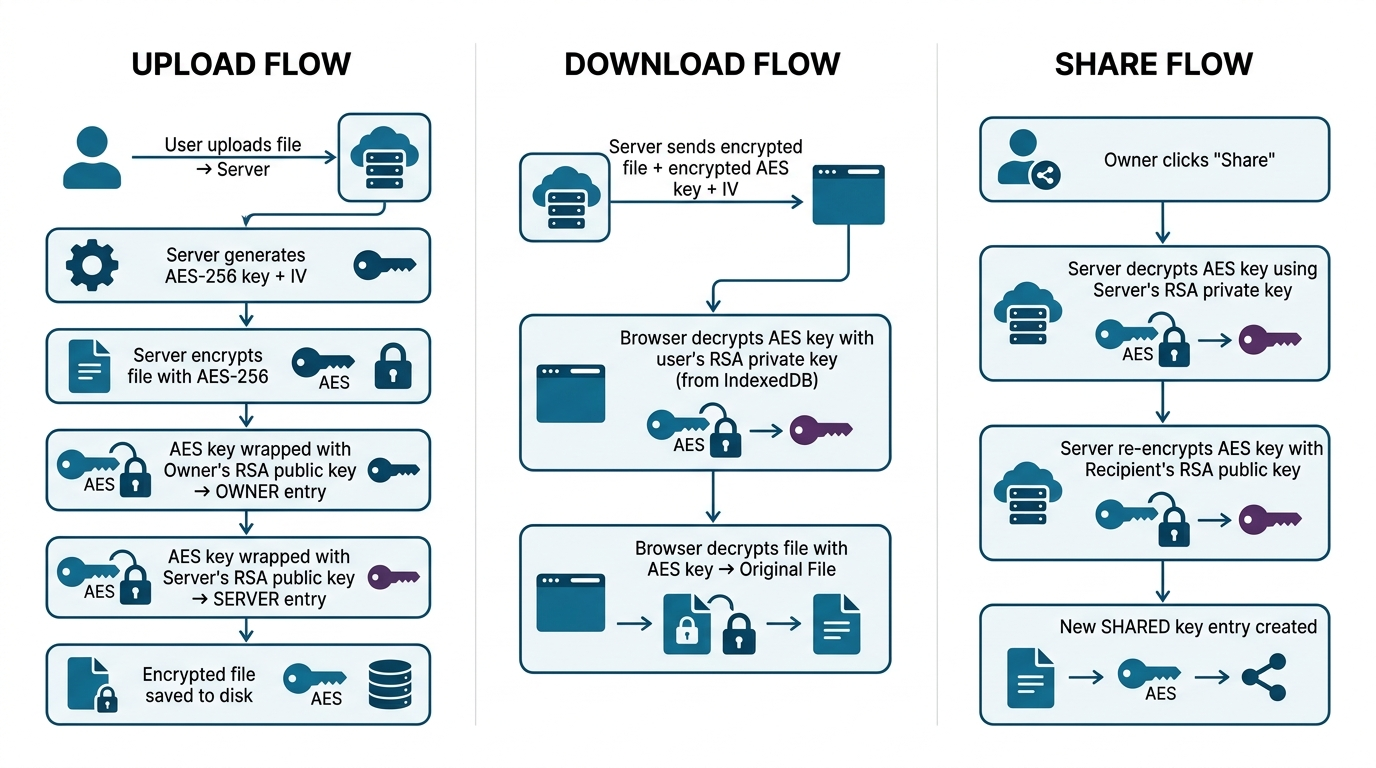
\includegraphics[width=\textwidth,height=0.78\textheight,keepaspectratio]{workflow.jpg}
\end{center}
\end{frame}

\begin{frame}{Demo --- Login \& Registration}
\vspace{-0.3cm}
\begin{columns}
\begin{column}{0.48\textwidth}
\begin{center}
\textbf{Login Page}\\[0.1cm]
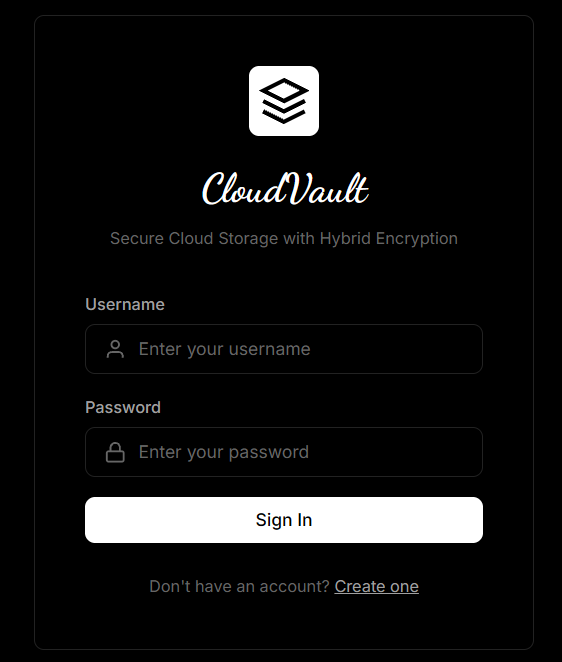
\includegraphics[width=\textwidth,height=0.55\textheight,keepaspectratio]{images/screenshot_login.png}
\end{center}
\end{column}
\begin{column}{0.48\textwidth}
\begin{center}
\textbf{Register Page}\\[0.1cm]
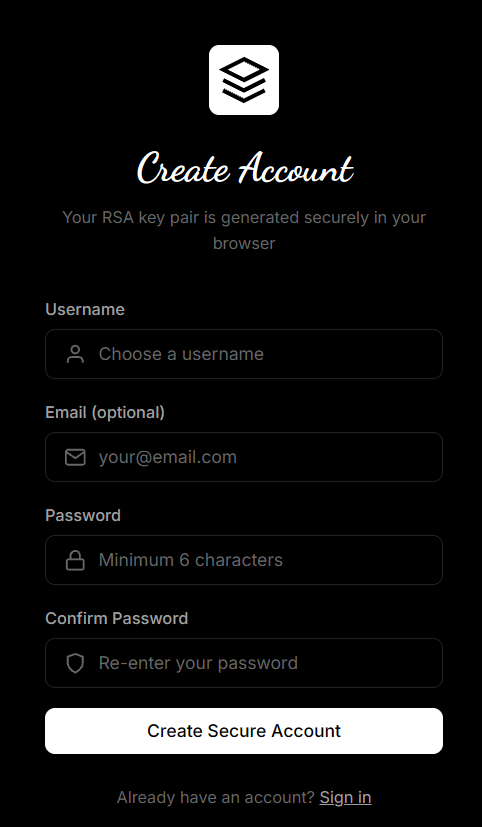
\includegraphics[width=\textwidth,height=0.55\textheight,keepaspectratio]{images/screenshot_register.png}
\end{center}
\end{column}
\end{columns}
\end{frame}

\begin{frame}{Demo --- Dashboard}
\vspace{-0.3cm}
\begin{center}
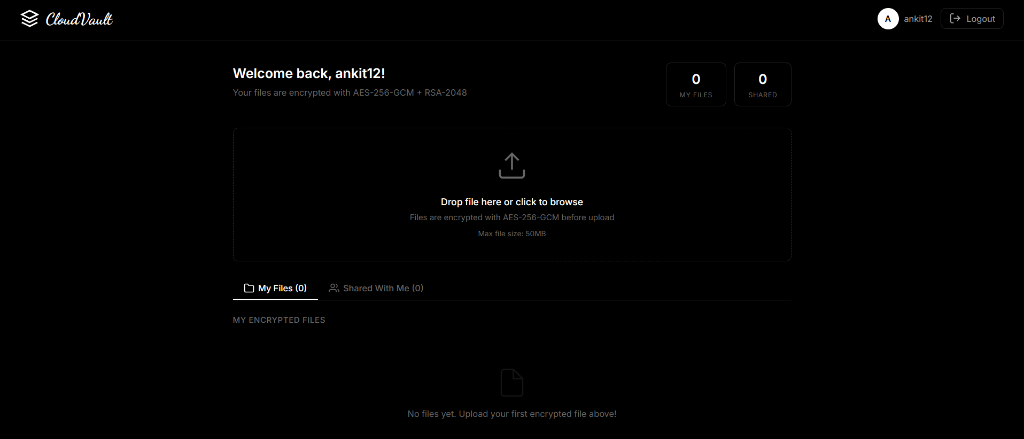
\includegraphics[width=\textwidth,height=0.65\textheight,keepaspectratio]{images/screenshot_dashboard.png}
\end{center}
\end{frame}

% ============================================================ %
%       SECTION 4: ANALYSIS                                    %
% ============================================================ %
\section{Analysis}

\begin{frame}{Performance Analysis}
\begin{block}{Measured Results}
\small
\begin{tabular}{@{}ll@{}}
\textbf{Operation} & \textbf{Performance} \\[0.2em]
RSA-2048 key generation (browser) & Under 1 second \\[0.2em]
File encryption (under 50 MB) & Near-instantaneous \\[0.2em]
Client-side AES decryption & Near-instantaneous \\[0.2em]
RSA key unwrapping & Under 100 ms \\[0.2em]
File sharing (key re-encryption) & Under 200 ms \\[0.2em]
JWT authentication overhead & Negligible \\
\end{tabular}
\end{block}

\vspace{0.2cm}
\begin{exampleblock}{Observation}
Hybrid encryption adds minimal overhead --- the AES key is only 32 bytes, so RSA operations on it are extremely fast.
\end{exampleblock}
\end{frame}

\begin{frame}{Security Analysis}
\begin{block}{Multi-Layer Security}
\small
\begin{tabular}{@{}ll@{}}
\textbf{Layer} & \textbf{Mechanism} \\[0.2em]
Passwords & BCrypt hashing with random salt \\[0.2em]
Sessions & Stateless JWT tokens (24h expiry) \\[0.2em]
API Protection & Spring Security filter + JWT validation \\[0.2em]
Files at Rest & AES-256-GCM encrypted on disk \\[0.2em]
Key Protection & RSA-wrapped AES keys per user \\[0.2em]
Client Keys & RSA private key in browser IndexedDB \\[0.2em]
Server Keys & RSA key pair auto-generated at startup \\
\end{tabular}
\end{block}
\end{frame}

\begin{frame}{Threat Analysis}
\begin{block}{Threats Mitigated}
\begin{itemize}
  \item \textbf{Server breach}: Attacker gets encrypted files + wrapped keys $\rightarrow$ cannot decrypt without user's RSA private key (stored only in browser)
  \item \textbf{Network interception}: JWT auth + encrypted file transfer $\rightarrow$ raw file never travels over the network
  \item \textbf{Unauthorized access}: Spring Security blocks all unauthenticated API calls
\end{itemize}
\end{block}

\begin{alertblock}{Known Limitation}
Clearing browser data deletes the RSA private key. A key export/backup feature is recommended for production.
\end{alertblock}
\end{frame}

% ============================================================ %
%       SECTION 5: INNOVATION & TECHNICAL CONTRIBUTION         %
% ============================================================ %
\section{Innovation \& Technical Contribution}

\begin{frame}{Innovation --- What Makes CloudVault Unique}
\begin{block}{Key Innovations}
\begin{enumerate}
  \item \textbf{Browser-Only Private Keys}: RSA private key is generated and stored exclusively in the browser (Web Crypto API + IndexedDB). The server \alert{never} sees it.
  \item \textbf{Zero-Effort Sharing}: Files are shared without re-encrypting the entire file --- only the AES key is re-wrapped using the recipient's RSA public key.
  \item \textbf{Hybrid Encryption with Key Envelope}: Each file has per-user encrypted key entries (OWNER / SERVER / SHARED), enabling granular access control.
  \item \textbf{Client-Side Decryption}: The original file is reconstructed entirely in the browser --- the server only delivers ciphertext.
\end{enumerate}
\end{block}
\end{frame}

\begin{frame}{Technical Contribution}
\begin{block}{Contributions to Cloud Security}
\begin{itemize}
  \item Demonstrated a \textbf{practical hybrid encryption model} for web-based file storage using standard browser APIs
  \item Implemented a \textbf{Key Envelope Table} design pattern for multi-user encrypted file access
  \item Achieved \textbf{zero-knowledge file sharing} where the server facilitates sharing
  \item Built a \textbf{full-stack reference implementation} using modern frameworks (Spring Boot 3 + React 19 + Web Crypto API)
\end{itemize}
\end{block}

\vspace{0.2cm}
\begin{exampleblock}{Tech Stack}
Spring Boot 3.2.5 (Java 17) | React 19 + Vite 8 | Web Crypto API | JWT | AES-256-GCM | RSA
\end{exampleblock}
\end{frame}

% =================== 6: REFERENCES =================== %
\section{References}
\begin{frame}{References}
    \nocite{*}
	\bibliography{reference}
	\bibliographystyle{unsrt}
\end{frame}

% =================== THANK YOU =================== %
\begin{frame}{}
\begin{center}
\vspace{2cm}
{\Huge \textbf{Thank You}}
\end{center}
\end{frame}

\end{document}

